
\chapter{概述}
\label{chap:intro}

\section{设计理念}
\label{sec:dongji}

本系统的设计与实现是天津大学图书馆建立学术科研和教育教学提供支撑系统体系的一部分。原本要设计的是一个高校机构库管理系统。主要功能是收集并整理本校老师和博硕士的科研成果,并组织分类后通过统一的发布平台进行展示。要实现的功能对本校科研水平展示和对本校学术资源的收集。但是通过对厦门大学和中科院等国内知名机构库系统的调研后发现:
\begin{enumerate}
\item 老式机构库系统从访问量上并没有达到预想的效果。由于现在更多的人习惯使用搜索引擎,博客等渠道作为获取信息的主要途径。所以目前国内主要的高校机构库平台访问量都不理想。基本上属于 “信息孤岛” 状态。
\item 老式机构库从内容的管理比较繁琐,信息实时性差,更新费时费力。由于老式机构库从结构上依然属于信息资源管理系统(erp),由于管理类系统的操作界面相对复杂,加之信息录入工作比较繁琐,所以大多老师学生不愿意使用。所以其主要的建库和信息维护工作还是需要由,机构库的管理部门(比如图书馆)来完成,而这些部门需要维护的信息来源却是学校里的教授或者学生。这就出现了信息多次传递的问题。带来的后果自然是管理部门费时费力,教授和学生不满意。
\item 老式机构库从系统实现上国内还是以dspace,Eprints,超星等平台为主,其内容的实现机理也是基本上面向数据存储的。这就给信息的结构化扩展带来了很多问题。
\end{enumerate}
除了以上列出的几个方面的问题以外,老式机构库追究其问题的根源是:这些系统是面向信息收集和信息管理部门而设计的。其更多的考虑了信息如何收集和展示。而忽略了信息来源(即老师和学生)在系统中的作用。管理部门更像实在自说自话,不断的向一个很少有人访问的门户网站上添加内容。而更加悲剧的是甚至这些信息的创作者有时都不知道还有这么一个平台上有他们写的东西。这种有着强烈web 1.0味道的应用在当今这个时代是必然会被淘汰的。

由于考虑到以上诸多问题,所以本系统开发之初即转换了设计理念。放弃了机构库面向信息收集、管理、发布为主要目标的设计,采用了面向信息创作者,为信息创作者提供便捷易用的个人文档管理平台为主要目标的设计理念:
\begin{itemize}
\item 系统主要的使用者是本校教师和学生。他们是系统主要的信息提供者
\item 以帮助教师和学生提高工作效率为首要目标。系统功能以实际出发帮助他们解决个人文档管理中的实际问题。
\item 由于教师和学生不是专职的信息管理人员,所以要系统必须提供简单易用的使用界面,上手使用必须无需任何额外的学习过程。
\item 系统信息组织不再以集中式的信息收集为主,而是把系统信息以个人文档的形式保存在每个人的私有空间下,每个用户决定这些文档的公开程度和公开范围。
\item 由于系统是面向个人的,所以系统不仅要成为个人文档的存放平台。还要成文个人文档的建立平台。所以系统的功能也更多的偏向于‘纯文本编辑’功能。
\item 如果本系统可以被广大师生接受并大量使用。那么把个人空间内公开的文档整理并展示将不是非常困难的事情,可以说是顺理成章的事情。所以本系统具有老式机构管理库绝大多数功能。
\item 信息管理部门和学校其他职能部门虽然不再是管理信息的主要角色。但是在本系统中他们可以为教师和学生提供类似“信息补全” “成果认证” 等一系列的服务。让用户可以更好的使用系统。
\end{itemize}
通过上面的描述,可以看出本系统的主要设计理念是“面向用户”而非“面向系统”。这一点理念上的变化有点像web 1.0到web 2.0的变化。由门户网站到博客、微博、个人空间的变化。如果用一句话来概括本系统的设计理念的话,应该是“如果用户可以在我们的帮助下把自己的文档和成果管理好,那么我们就可以帮助他们更好的提升并展示自己”。还需要解释的是:由于系统设计理念的不同,所以这套系统在命名上也不再沿用“机构管理库”这样的名词。从功能上主要以管理个人文档和成果为主,所以暂时以“个人学术文档服务平台”命名。

刚才提到系统要以帮助教师和学生解决个人文档管理中遇到的问题为主要目标。那么到底在现在高校中老师和同学们在教学科研和学习中都有那些问题急需解决呢?我们将在下一个小节来汇总一下。

\section{要解决的问题}
\label{sec:question}

上一节提到本系统的设计理念是:帮助每一个用户解决个人文档管理中遇到的问题为主,收集和展示文档资源为辅。现在我们就来分析一下当今高校教师和学生在管理个人文档方面都有哪些问题:
\begin{enumerate}
\item 无论是学术成果的期刊论文、学生的毕业论文、个人编著的书籍、项目的申报和评审材料、技术报告书、教学演示文稿等学术性文档,还是个人的工作笔记、项目日程计划、工作日记等普通文档。在当今高校中,制作这些文档的主要工具是microsoft的office系列软件。office系列软件有“所见即所得”、“易于上手”等诸多优点,在目前社会(起码在中国)上也有相当大的用户群和相当高的普及率,其中以word软件使用频率最高。但是word软件给我们带来的便捷也是有一定局限性的,使用word一段时间以后就会发现它有如下缺点:
  \begin{description}
  \item[难以专心] 写Word文档的时候,我们经常浪费大量时间在Word本身上,特别是那80\%我们用不到的功能。有时看似非常智能的功能,使用起来却有可能成为麻烦的开始。比如项目列表自动添加序号功能,就经常给我们添加一些无用的序号,我们还要费力去删掉它。
  \item[浪费时间在排版上] 使用Word时,我们会花费大量力气去排版,试图让文档变得漂亮一些。是粗体还是斜体,是宋体还是黑体,对创作来说这根本不重要。据了解,一个学生在写作一篇学位论文的过程中用来使用word进行排版格式的时间至少要5个小时。这还是对于一个word操作的熟练的人来说。毫不夸张的说,写毕业论文过程基本就是一个学习word操作的学习过程。
  \item[重复学习成本高] word版本更近快速,从2003,2007,再到2010,每个版本的菜单设置和操作习惯都有所变化,其中以03到07的变化最大,甚至文件格式都不再相同。这样就给用户带来很到的重复学习的成本,好不容易学会来一个版本的操作,下一个版本就出来了,而且操作习惯完全不同。不想升级还不行,因为文件格式的原因,别人用新版本写的文档老版本用户打不开。
  \item[不适合编辑大型文档] word用来排版一些工作报告,宣传册等小型的文档是比较合适的,但是如果用它来编辑学位论文,书籍等大型文档的时候。不仅其所谓的“所见及所得”特性不能完全发挥作用。而且其来带的附加操作会非常的“重”。
  \item[不适合编辑科技文档] word对于编辑以文本格式为主的文档时,可以发挥其特性。但是在编辑科技类文档时,文档的内容就不单纯只用文字了,它会包括数学公式、化学分子式等复杂格式。word在处理这些格式的文本时,其排版的能力就确实一般了。不仅需要安装公式编辑器等插件才可以使用,而且制作好的文档在不同机器上打开时,其样式可能会变得面目全非。
  \item[文档格式封闭] 众所周知,word作为一款闭源软件,用它编辑出来的文档的内部格式是可见的。虽然在07版本之后这种情况有所好转,但是其开放的友好程度依然不好。这样的格式带来了很多问题,首先,封闭格式为二进制文件,而非内容原本,这样就不易做版本控制。其次,封闭格式不易在网络上传播,众所周知,word文档无法在网络上直接查看和编辑,即使复制粘贴成web格式,其格式也会不预期的变化。在这个互联网如此普及的时代,缺失这个特性是非常不方便的。
  \item[价格昂贵] 需要说明的是,这个问题在我国并不是什么真正的问题。首先,word盗版很好获取,我们可以免费的使用这款收费软件。其次,值得称道的是,在我们的高校里,学校已经为我们花钱购买了正版的office系列软件。这样,我们不仅可以免费使用,而且也不用背上“盗贼”的恶名。
  \end{description}
综上所述,word软件的使用给我们的文档编辑带来很多便利,但是对于某些特殊的场合,特别是编写学术性文档的时候,它也未必是我们最佳的选择。总之,无论那种类型的文档,更多的关注文档的内容而非文档的格式和排版,应该是我们创作的最终目标,也是本系统要帮助用户解决的第一个问题。下一个小节中,我们将介绍如何利用\smarkdown和\LaTeX来帮助用户更少的关注排版格式,通过更低的学习成本,更好的完成个人文档的创作。
\item 文档保存存在安全隐患,文档管理效率低下。上文提到几乎在现今高校,几乎所有的学术性文档和个人普通文档几乎都由office系列软件进行编辑,由此也就带来了另外一个问题:在文档的保存上,几乎所有的文档都以doc、docx、ppt、pptx等格式保存在个人电脑的硬盘中。因为个人电脑硬盘几乎不具备冗余数据保护功能,由于个人电脑硬盘故障而造成的文档丢失事件屡见不鲜。加之有些用户在日常工作中没有好的文档管理习惯,很多文档都直接保存在系统桌面上,而且没有备份文件。这样当系统崩溃或者硬盘故障的时候,真的是欲哭无泪了。

这种文档保存方式的另外一个弊端是:文档管理和查找非常的费时费力。众所周知,随着个人电脑中各式文档数量的增加,组织管理这些文档确实是一个比较具有挑战性的工作,不仅会耗费大量的时间来组织目录,而且随着目录的增多和加深,查找文档将非常不方便。由于office文档格式封闭,所以想要进行全文检索几乎不可能,而且windows也没有提供文件标签查找的能力,所以只能单靠文件名来进行查找。如果当时给文件起名的时候有一点疏忽写错或者省略了部分内容,那么就会面临明知道文件在硬盘中却找不到的窘境了。

固然,有好的文档行管理习惯的人,可以把系统目录结构分的很细致,并且保持好的文件命名方法,但是即使这样再有些情况下管理文件依然很费力。比如:文件a属于项目A,所以它应该被放置于文件夹A下面,如果文件a又是个人学习的一个必要文件,所以也应该放入个人学习的目录中。为了从不同的角度都可以很方便的查找到该文件,我们不得不把文件a分别存入两个目录。这样又会带来文件更新与版本不统一的问题。使用快捷方式更不可取,因为文件夹被移动后链接就失效了。
\item 文档缺少版本控制,备份文件管理混乱。每一个大型文档的写作都需要经历若干个版本。如何保存和管理好这些“中期成果”就成为来很棘手的问题。有人喜欢在文件名后加上日期来保存这些文件,但是单纯的日期也无法描述当日所做的修改,只好再把简短的修改日志写在文件名中。这样日积月累,我们就有保存来很多拥有很长很长文件名的文件,不仅浪费空间,而且不易查找和使用。这些还不是问题的全部,把备份考虑进来以后,问题就变得更加复杂。

不把鸡蛋放在一个篮子里是一个必要的常识。显然,保持良好的备份习惯是避免文件丢失而造成无可挽回损失的必要条件。但是文档的备份必然又会让用户的文档管理工作更加复杂。比如:一般情况下,我们的文档保存三个备份,应该可以确保其安全。这三个备份分别保存在三台不同的计算机中,现在且不讨论加之文件的中间版本文件后这种管理模式有多么复杂,单纯保持这三个备份一致的状态就是一个非常费时费力的事情。有时不小心使用来没有被更新过得文件进行编辑和使用,必然要造成工作时间上的浪费和个人智慧成果的丢失。
\item 文档在多设备间同步困难,难以发挥现在移动设备带来的便利。对于现代人,拥有一台以上的电子计算机已经是非常普遍的了。在高校,几乎每个老师会在办公室和家里个有一台电脑,加上日常出差开会可能还会有一台笔记本电脑。多台电脑虽然给我们带来来方便,但是也引发了一些问题。比如:很多老师需要在家继续完成办公室未完成的工作。这就需要把单位电脑上未完成的文档,复制到家里电脑上(比如用U盘)。工作后还需要把文档再复制回去。如果某一天忘记复制文件了,那么在家就没有办法工作了。而且文件来回复制有时会造成版本的混乱,往往会造成部分工作成果的丢失。

当今手机和平板电脑的普及让我们的生活,特别是娱乐生活得到来很到程度的进步。平时我们可以使用手机进行上网,阅读,游戏等活动,但是使用这些移动设备来编辑、查看我们的个人文档的人却不多,尤其是学术性文档。其中一个重要原因就是文档在不同设备间的传递存在不便利性:
  \begin{description}
  \item[电脑和电脑之间] 如果两台电脑在一个局域网(往往一个实验室内),采取的传递方法多为“windows共享”,“飞鸽传书这样的局域网工具”等,而在不同网段的机器间,就只能靠“ftp服务”,“qq文件传输”这样的服务。如果在教育网主机和公网主机间传递文件,有时限于网速的限制,往往是使用u盘来的更好一些。
  \item[电脑和移动设备间] 由于移动设备使用的操作系统的不同,其传递文件的应用也不尽相同。此类应用虽然很多,功能也五花八门,单其基本原理也无非是通过局域网,或者蓝牙功能进行传输。其实目前最为广泛使用的还是把移动设备通过数据线链接到电脑上进行复制粘贴。
  \end{description}
综上所述,无论是电脑与电脑间,还是电脑和移动设备间,要想传递文档,多少还是需要一些“被折腾”的操作的(起码也要把数据线找出来)。
\item 文档分发方式原始。什么叫文件分发,比如:一个老师讲课后,同学们想要老师讲课的课件。这个时候老师的课件就需要分发到每一位同学手中。据调查,目前比较普遍的分发方式以使用u盘直接复制和老师提供公共邮箱(告诉同学一个邮箱的地址和密码)下载地址为主。这两种方式可以说相当原始,而且存在很多问题。所以目前普遍缺少一种可以把一份文件分发给特定人群的应用。
\item 项目文件和数据分散在不同项目组成员手中,管理胡乱。对于一个项目的文件的管理更是对文档管理的一个大的挑战,一个项目从构思开题,到结项总结。其中包含众多的文档和数据,而且这些文档和数据多数情况下会有不同的建立者。在拥有很多项目组成员,而且每个人手中都有项目相关文件的时候,如何把一个项目所设计的所有的文档数据保存好,管理好,确实是一个相当大的课题。旧有的文档管理模式必然会造成管理的混乱和数据文档的丢失。比如经常会出现这样的情况:项目负责人在项目要中期检查的时候需要参考项目建立之初时某些文档的内容,而这些文档的建立者是项目组其他的成员,而改文档的最新版本在他手中,而由于某些项目的时间线会拉的很长,所以中间该成员有可能会因为各种原因找不到该文档。显然文档管理上的混乱造成了时间和精力上的浪费。这还不是问题的全部,更严重的情况是有可能的项目数据的丢失,文档可以重新创作,而实验数据的丢失将造成灾难性的后果。
\item 教师和学生的研究方向,研究内容,研究成果等信息难以被了解。现在如果在校园里随便找几个学生,问一下他们自己学院本专业的老师都有谁,也许有大部分学生都能回答,如果问他们这些老师的研究方向,他们或许也知道一部分。但是如果深入的问这些老师有那些成果他们在自己研究方向上具体做来哪些工作,那么大部分学生就未必能回答上来了\footnote{对此问题并没有做科学的调查统计,此处结论可能有误}。由此证明,在当今高校,缺乏对教师的研究近况进行展示和了解的平台。以我校\footnote{天津大学}为例,如图~\ref{fig:xfig1}所示\footnote{图为学院为本文作者导师的个人简介页},学校主页上提供的老师的个人介绍只有一个简陋的静态网页。本校学生甚至其他学校学生或者社会上的人要想更多的了解一个学校老师的科研成果,研究近况,个人魅力等信息,甚至要和这些老师进行交流或者向老师请教学术问题,就需要建立更强大的成果展示平台和学术交流平台。
\begin{figure}[H] 
  \centering
  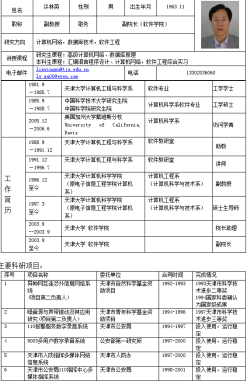
\includegraphics{xuly}
  \caption{导师个人介绍}
  \label{fig:xfig1}
\end{figure}
综上所述,在高校,教师和学生在日常的个人文档的建立,管理,分发,传播等方面确实存在着一些问题,这些问题虽然经过多年的适应过程,表面看上去并不是不可以被接受,有时也会被认为是“本应如此”的事情。但是,仔细想想我们平时浪费在调整格式、管理文档、寻找文档、同步文档中的时间是否积压了我们考虑问题和科学实验的时间呢?如果通过某些手段使我们避免这些时间的浪费,我们的教学与科研是否会更有效率呢?

本章简单介绍了本系统的构建缘由,设计理念和要解决的问题。下一章,我们将针对以上提出的每一个问题,介绍本系统的相应的应对方案。并由此引出本系统的总体架构设计。
\end{enumerate}